\chapter{Data Mining}
\label{cha:data_mining}

After preprocessing the data, the next step is to build a classifier to predict the success of a movie. To find the best classifier a set of different algorithms is evaluated:
K-Nearest Neighbor, 
Na\"{i}ve Bayes, 
Support Vector Classifier, 
Neural Net, 
Decision Tree and 
Random Forest.

The first goal of the analysis was to predict the success in four different classes. Since an analysis in that detail with the given data set is very unprecise, a binary classifier was created.
For all of the named algorithms an individual feature selection is applied to get the best results. The important features are selected by a greedy feature wrapper. This feature wrapper starts with the full set of features and drops features as long as the result improves. The results are checked with a stratified 10- fold cross-validation. Additionally to the selection of features, filters for features like the number of actors and number of production companies can be applied. For example actors, directors and companies, which are not frequently participating in the movie-production-scene can be eliminated. Thus it can be assured that only columns are taken into account which are contained in a reasonable amount of movies, and therefore have an impact on the classifier. \\
In the next step some hyperparameter tuning is needed to improve the classifiers. To find the best parameter setting, a grid search in combination with a 10-fold cross-validation, scoring the highest F1-score (macro), is applied to the classifiers.
The achieved F1-scores of the three best binary classifier are listed in table \ref{tab:binary_classifier}. 

Previous tests using the micro F1-score have shown, that even though promising results could be scored, the classifiers only learned guessing in this setting. Therefore the F1-score had been changed to macro.
%At first the classifiers are scoring the micro F1-score. Even though the result looks promising at the beginning, the classifier are mostly guessing the majority class in this setting. For that reason every classifier is scoring on the macro F1-score.
 Since the data set for the binary classifier is unbalanced with a ratio of 75\% "successful" and 25\% "unsuccessful". The next step to improve the classifiers is to balance the train set. That for the stratified cross validation is used to balance the train set. For further improvement the train set can be downbalanced by shrinking the majority class to the size of the minority class. But since the data set is already quite small after the preprocessing, the downsampling worsens the classifiers. To not shrink the dataset any further upsampling can be used to increase the minority class of the train set to the size of the majority class. In the following section the the two best performing classifiers - k nearest neighbor and support vector classifier - are examined in more detail.
\begin{figure}[h]
	\center
	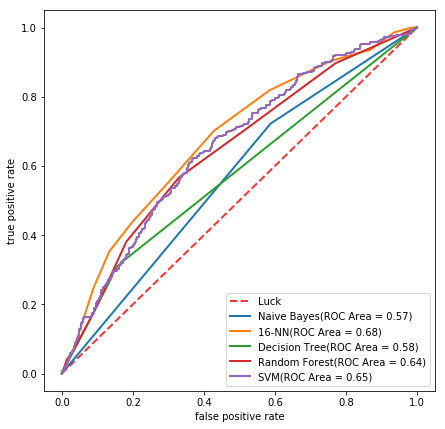
\includegraphics[width=0.7\textwidth]{images/roc.png}
	\caption{Macro average ROC Curves for all classifiers}
	\label{img:roc}
\end{figure}
 
%\begin{center}
%\begin{table}
%	\begin{tabular}{ | p{3.5cm} | p{1.5cm} | p{1.5cm} | p{2cm} | p{2cm} |}
%    \hline
%    Algorithm & F1 Macro & F1 Micro & Downsampled Macro  & Downsampled Micro\\ \hline
%    Decision Tree & 56.5\% & 75.5\% & 61.9\% & 63.0\% \\ \hline
%    Random Forest & 58.7\% & 76.0\% & 80.6\% & 81.5\% \\ \hline
%    Support Vector Classifier & 56.5\% & 75.0\% & 60.7\% & 60.8\% \\
%    \hline
%    \end{tabular}
%    \caption{Binary Classifier Results} 
%   \label{tab:binary_classifier}
%\end{table}
%\end{center}
\section {Classifiers}
\paragraph{K nearest neighbor}
After the preprocessing the data set is highly dimensional with more than 50,000 columns. Even though kNN does not work very well on a high dimensional data set, the algorithm is the best performing one with a good feature selection. After dropping all the actors, country, genre and quarter information and limiting the director and the companies to the ones that took part at at least three movies of the data set, the algorithm scores an F1 score of 61.4\%. The algorithm is comparing the labels of the 16 nearest neighbors calculated with the euclidean distance. Both down- and upsampling worsens the classifier. 

\paragraph{Support Vector Classifier}
As the kNN the support vector classifier works best after dropping a lot of features. Without any information to the actors, country, quarter, genre and age limitation and limiting the companies and directors to the ones that took part at at least three movies, the classifier scores an F1 score of 60.7\%. For the best result the algorithm works with a linear kernel and a balanced class weight. Both down- and upsampling worsens the classifier.

%\paragraph{Decision Tree}
%One way to deal with the issue of an unbalanced data set is to use a tree-structured classifier, since the hierarchical structure allows them to learn signals from both classes.
%To find the best parameter setting for the decision tree the grid-search tests the parameters split criterion, max depth, minimum samples to split and the class weight in a ten fold cross-validation. After dropping the "quarter", "runtime" and "adult" columns, the classifier scores without any sampling, no class weight, an entropy split criterion and a max depth of 100 an F1 score of 58\%. Both the down- and the upsampling worsens the classifier.

%\paragraph{Random Forest}
%Like the decision tree, random forest builds  a hierarchical structure, which can handle unbalanced data sets better than other algorithms. In addition it corrects the overfitting habit of a decision tree. In the gridsearch hyperparameters like the split-criterion, number of features, the minimum sample to split and whether bootstrap samples are used or not are evaluated. After dropping the actors and the release quarter, the classifier scores a F1 score of 59\%. As with the decision tree neither down- nor upsampling the train set improves the result.
\section{Evaluation and Prospect}
\paragraph{Evaluation}
\label{cha:prospect}
As discovered in the previous paragraphs, some classifiers perform better than others. One reason could be seen in the dataset. The final dataset of about ~3900 rows can be considered as relativly small. Therefore, as shown in the ROC Curves above, Decision Tree and Random forrest are not performing the best scores. Usually they are rely on large data set, where they can evaluate data more efficiently. The Random forest however, scores an higher accuracy since it takes knowledge from various trees inside the forest.

Other classifiers as for example Na\"{i}ve Bayes perform not as well as the trees. One possible reason could be that Na\"{i}ve Bayes assumes that no correlation between the features exist. However, in this specific task movies with more famous actors usually generate a bigger budget. 







%\begin{itemize}
%	\item very small dataset -> not all algorithms perfom very well
%	\item Example numbers -> some perform better: why? 
%	\item Analysis of values
%\end{itemize}

